%%%%%%%%%%%%%%%%%%%%%%%%%%%%%%%%%%%%%%%%%%%%%%%%%%%%%%%%%%%%%%%%%%%%%%%%
\chapter{Background}\label{chap:background}
%%%%%%%%%%%%%%%%%%%%%%%%%%%%%%%%%%%%%%%%%%%%%%%%%%%%%%%%%%%%%%%%%%%%%%%%

\begin{center}
	\begin{minipage}{0.8\textwidth}
		\begin{small}
			This chapter provides the required theoretical background, and literature review and states the research questions in context.
		\end{small}
	\end{minipage}
	\vspace{0.5cm}
\end{center}

\minitoc

%%%%%%%%%%%%%%%%%%%%%%%%%%%%%%%%%%%%%%%%%%%%%%%%%%%%%%%%%%%%%%%%%%%%%%%%
\section{Theoretical Background}\label{sec:theobackground}
%%%%%%%%%%%%%%%%%%%%%%%%%%%%%%%%%%%%%%%%%%%%%%%%%%%%%%%%%%%%%%%%%%%%%%%%
The required theoretical concepts to understand the rest of the manuscript are briefly described in the following subsections.

%%%%%%%%%%%%%%%%%%%%%%%%%%%%%%%%%%%%%%%%%%%%%%%%%%%%%%%%%%%%%%%%%%%%%%%%
\subsection{Convolutional Neural Network}\label{sec:CNN}
%%%%%%%%%%%%%%%%%%%%%%%%%%%%%%%%%%%%%%%%%%%%%%%%%%%%%%%%%%%%%%%%%%%%%%%%
Convolutional neural network (CNN) is a kind of neural network that simulates some actions generated in the human visual cortex using convolution mathematical operation to extract features from input and pass these features through successive layers to generate more abstract features to yield a final output \cite{726791}. It processes data having grid patterns (images for example) and learns spatial feature hierarchies adaptively and automatically, from basic to complex patterns \cite{yamashita2018convolutional}. 

Feedforward neural networks, also called deep feedforward networks, or multilayer perceptrons (MLPs), are classic examples of neural networks \cite{Goodfellow-et-al-2016}. A mathematical representation of a biological neuron is called a perceptron \cite{mcculloch1943logical}. Figure \ref{fig:neuron} the representation of a biological neuron. While the axons of other neurons provide electrical signals to the dendrite in actual neurons, these electrical signals are represented as numerical values in perceptron. Electrical impulses are regulated in various amounts at the synapses between the dendrite and axons. The perceptron models this by multiplying each input value by a value referred to as the weight. Soma also called the cell body is responsible for input processing and decision making in a biological neuron. Only when the sum of the input signals is greater than a predetermined threshold does a real neuron really fire an output signal. By computing the weighted sum of the inputs, which represents the entire strength of the input signals, and applying an activation function to the sum to determine the output, we may mimic this phenomenon in a perceptron. Nonlinear activation functions can be used for performing nonlinear transformations with perceptrons. Appendix Table \ref{tab:activations} lists some of the commonly used activation functions. Perceptron calculates the dot product between a learnable weight vector and an input vector and passes it through an activation function after adding a scalar bias term. Mathematically, the operation of perceptron can be represented as Equation \ref{eq:perceptron}.
\begin{equation}\label{eq:perceptron}
	y_{out}=f_{act}(\sum_{i=1}^{n}w_ix_i+b)
\end{equation} 
where $y_{out}$ is the output of the perceptron, $f_{act}$ is the activation function. $w_i$ is the weight corresponding to input $x_i$, and $b$ is the bias. Figure \ref{fig:perceptron} shows the schematic representation of a perceptron. MLP consists of many layers of perceptrons where each perceptron of a layer is fully connected to every other perceptron in the previous layer as shown in Figure \ref{fig:MLP}. Neural networks are trained using optimization algorithms. An optimization algorithm updates learnable parameters (weights, biases) of the network to minimize a task-specific loss function. Gradient descent \cite{Ruder2016} and its extensions like RMSprop \cite{tieleman2012lecture} and Adam \cite{Kingma2015} are some of the popular choices for optimization. We have used Adam optimizer in this study and Appendix Section \ref{app:optimizer} contains a brief overview of Adam optimizer. Interested readers are suggested to consult the study by Ruder \cite{Ruder2019Neural} for a detailed overview of gradient descent based optimization algorithms. Traditional MLPs are not well suited for image processing as they require a large number of parameters and can not take into consideration the spatial information in images. Although, modern MLPs like ResMLP \cite{touvron2022resmlp} have been customized for image classification tasks CNNs are preferred over them.


\begin{figure}[htb!]
	\centering
	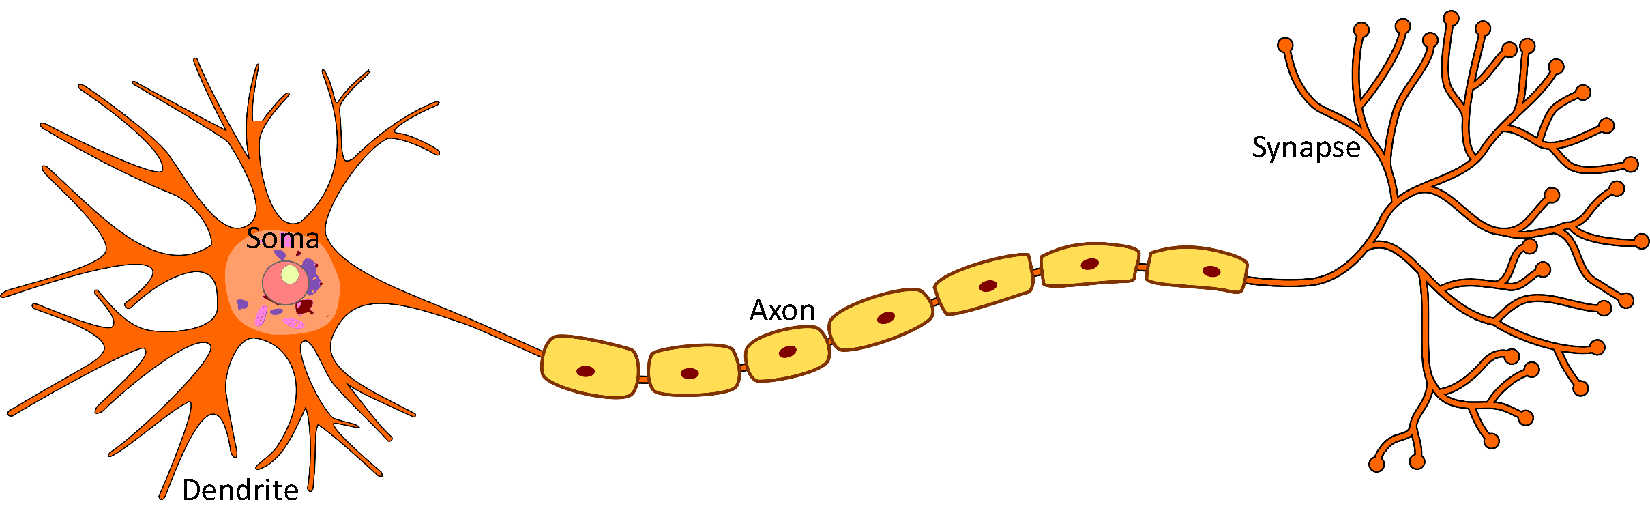
\includegraphics[width=\textwidth]{images/background/Neuron.pdf}
	\caption[Illustration of a biological neuron]{Illustration of a biological neuron. Image modified from \cite{Neuron}.}
	\label{fig:neuron}
\end{figure}
\begin{figure}[htb!]
	\centering
	\begin{subfigure}[b]{0.8\textwidth}
		\centering
		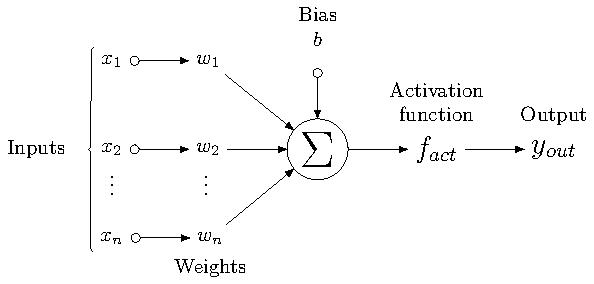
\includegraphics[width=\textwidth,keepaspectratio]{images/background/perceptron_perfect.pdf}
		\caption{Perceptron.}
		\label{fig:perceptron}
	\end{subfigure}
	\hfill
	\begin{subfigure}[b]{\textwidth}
		\centering
		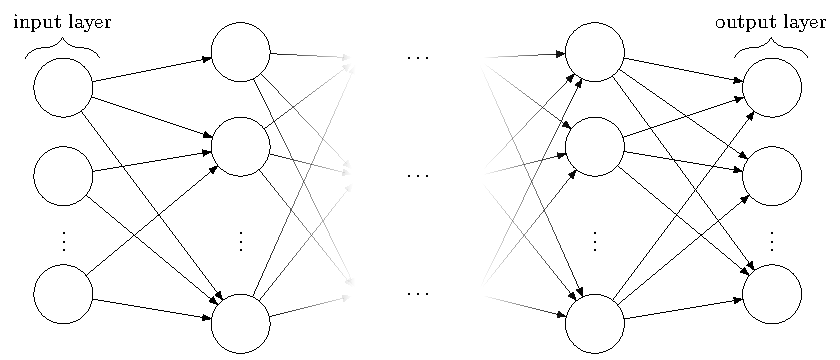
\includegraphics[width=\textwidth,keepaspectratio]{images/background/MLP.pdf}
		\caption{Multilayer perceptron (MLP).}
		\label{fig:MLP}
	\end{subfigure}
	
	\caption[Schematic representation of perceptron and multilayer perceptron]{Schematic representation of perceptron and multilayer perceptron (MLP). Images modified from \cite{Perceptrontex, MLPtex}.}
	\label{fig:percetron-mlp}
\end{figure}

The idea of convolution, a mathematical technique that entails swiping a tiny kernel over an image and computing the dot product between the kernel and the corresponding pixels in the image, serves as the foundation for CNNs. By spotting patterns in the data, this procedure aids in the extraction of features from the image. A feature map, which highlights particular aspects of the image such as edges, corners, and textures, is the result of this operation. The convolution operation is shown in Equation \ref{eq:conv1} \cite{Goodfellow-et-al-2016}.
\begin{equation}\label{eq:conv1}
	S(i, j)=(I * K)(i, j)=\sum_m \sum_n I(m, n) K(i-m, j-n)
\end{equation}
where $S$ is the output feature map, $I$ is the input image, $K$ is the kernel of size $m \times n$, $*$ represents the convolution operation, $i$ and $j$ are the row and column indexes of an element from $S$. The convolution is commutative, so the equation can be also written as:
\begin{equation}\label{eq:conv1}
	S(i, j)=(I * K)(i, j)=\sum_m \sum_n I(i-m, j-n) K(m,n)
\end{equation} 
Many deep learning libraries uses cross-correlation function in place of convolution as shown in Equation \ref{eq:cross-core}.
\begin{equation}\label{eq:cross-core}
	S(i, j)=(I * K)(i, j)=\sum_m \sum_n I(i+m, j+n) K(m,n)
\end{equation}
Cross-correlation is not commutative but has similar properties as convolution. A convolution operation on a two dimensional input image is illustrated in Figure \ref{fig:conv2dillustration}. Stride and padding are frequently used with convolution operation. Stride specifies how many pixels the kernel moves after each convolution operation i.e. the sliding of the kernel between the production of each output element. Padding is the process of adding empty pixels around the border of an input image. Padding is used to maintain image size and also for finding patterns in borders with full convolution on edge pixels.
To decrease the dimensionality of the feature maps and boost computing efficiency, CNNs use pooling layers in addition to convolutional layers. Downsampling is normally carried out by pooling layers using the maximum or average value of a set of adjacent pixels in the feature map as illustrated in Figure \ref{fig:poolingillustration}. Pooling also helps for making the model invariant to subtle translational changes in input. Convolutional, pooling, and fully connected layers are some of the layers of interconnected nodes that make up a CNN. The final classification or regression operation is carried out by the fully connected layers. Figure \ref{fig:CNN-schematic} shows a schematic representation of a CNN which stacks convolutional layers with an activation function applied after the convolution operation, pooling layers, and fully connected layers with activation functions.  Although, vision transformers \cite{Henry2022} are gaining a lot of popularity for various vision related tasks including medical imaging, modern CNN architectures like ConvNext \cite{liu2022convnet} and EfficientNetV2 \cite{EfficinetNetV2Ref} compete on par with them. Section \ref{sec:CNN-archis} contains brief descriptions of the CNN architectures used in this thesis.

\begin{figure}[htb!]
	\centering
	\begin{subfigure}[b]{0.8\textwidth}
		\centering
		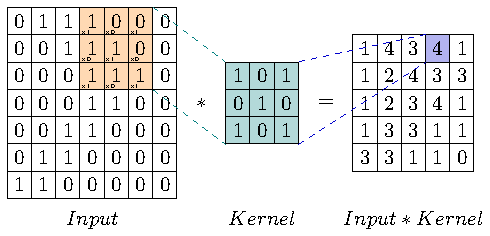
\includegraphics[width=\textwidth,keepaspectratio]{images/background/conv2d.pdf}
		\caption{Illustration of a convolution operation \cite{Conv2D}.}
		\label{fig:conv2dillustration}
	\end{subfigure}
	\hfill
	\begin{subfigure}[b]{0.7\textwidth}
		\centering
		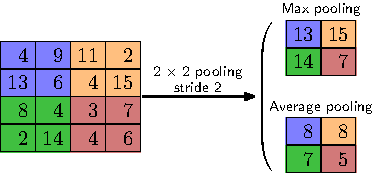
\includegraphics[width=\textwidth,keepaspectratio]{images/background/Pooling.pdf}
		\caption{Illustration of pooling operation.}
		\label{fig:poolingillustration}
	\end{subfigure}
	\hfill
	\begin{subfigure}[b]{\textwidth}
		\centering
		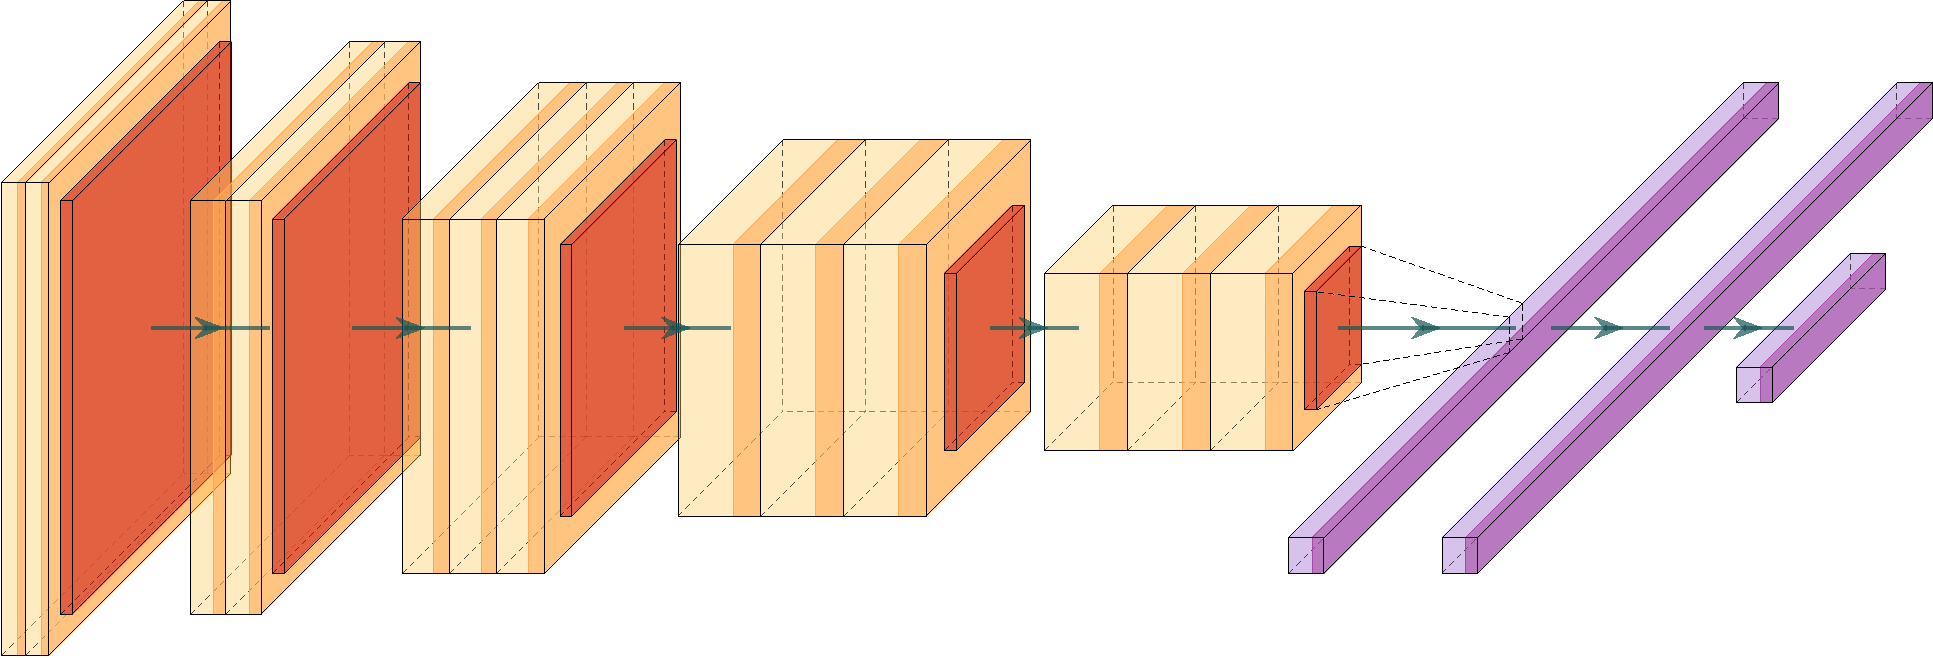
\includegraphics[width=\textwidth,keepaspectratio]{images/background/CNN-schematic.pdf}
		\caption{Schematic representation of a convolutional neural network. The yellow, and violet boxes with shaded endings represent convolutional and fully connected layers respectively with activation function. The red box represents pooling layer.}
		\label{fig:CNN-schematic}
	\end{subfigure}
	
	\caption{Schematic representation of convolution operation, pooling operation and convolutional neural network.}
	\label{fig:conv-CNN-schematic}
\end{figure}
%%%%%%%%%%%%%%%%%%%%%%%%%%%%%%%%%%%%%%%%%%%%%%%%%%%%%%%%%%%%%%%%%%%%%%%%
\subsection{Decision Tree}\label{sec:DecTree}
%%%%%%%%%%%%%%%%%%%%%%%%%%%%%%%%%%%%%%%%%%%%%%%%%%%%%%%%%%%%%%%%%%%%%%%%
Decision tree is a supervised learning algorithm, which can be utilized for both regression and classification tasks \cite{quinlan1986induction,BreiFrieStonOlsh84}. In this thesis, we are focusing on the decision tree for classification task. Decision tree represents a classifier as a recursive partition of instance space using a set of splitting rules \cite{quinlan1986induction,BreiFrieStonOlsh84}. These rules are easy to visualize and interpret with tree diagrams. Decision tree is a directed tree with no incoming edges at the root node and each of the other nodes has just one incoming edge. A decision or leaf or terminal node is a node without outgoing edges. All other nodes are called test or internal nodes. The instance space is divided into two or more sub-spaces by each test node based on a discrete function of input attribute values. Each decision node is given a class that corresponds to the best suitable target value. Instances are classified according to the test results by navigating from the tree's root to a leaf.

Figure \ref{fig:ex-dtree-dataset} shows an example training dataset and Figure \ref{fig:ex-dtree} shows the corresponding decision tree for deciding about playing golf (Yes/No) based on predictors like Outlook (Sunny/Overcast/Rainy), Temperature (Hot/Cool/Mild), Humidity (High/Normal), and Wind (Weak/Strong) \cite{DecTreeExample}. The red, yellow, and green boxes represent root, internal, and decision nodes respectively.
\begin{figure}[htb!]
	\centering
	\begin{subfigure}[b]{0.6\textwidth}
		\centering
		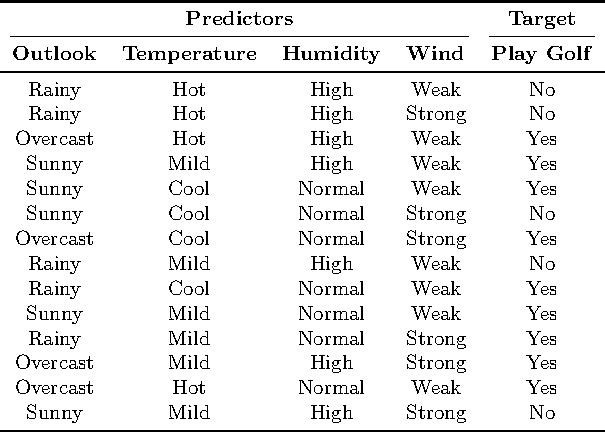
\includegraphics[width=\textwidth,keepaspectratio]{images/background/Decision_Tree_Table.pdf}
		\caption{Training dataset.}
		\label{fig:ex-dtree-dataset}
	\end{subfigure}
	\hfill
	\begin{subfigure}[b]{\textwidth}
		\centering
		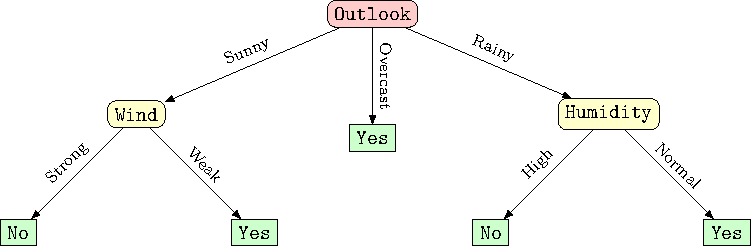
\includegraphics[width=\textwidth,keepaspectratio]{images/background/decision_tree_new.pdf}
		\caption{Decision tree.}
		\label{fig:ex-dtree}
	\end{subfigure}
	
	\caption[An example of decision tree]{An example of a decision tree for deciding about playing golf (Yes/No) based on predictors like Outlook (Sunny/Overcast/Rainy), Temperature (Hot/Cool/Mild), Humidity (High/Normal), and Wind (Weak/Strong) \cite{DecTreeExample}.  The red, yellow, and green boxes represent root, internal, and decision nodes respectively.}
	\label{fig:DecTreeExample}
\end{figure}

%%%%%%%%%%%%%%%%%%%%%%%%%%%%%%%%%%%%%%%%%%%%%%%%%%%%%%%%%%%%%%%%%%%%%%%%
\subsection{Formal Concept Analysis and Concept Lattice}\label{sec:FCA}
%%%%%%%%%%%%%%%%%%%%%%%%%%%%%%%%%%%%%%%%%%%%%%%%%%%%%%%%%%%%%%%%%%%%%%%%
Formal concept analysis (FCA) is a method of generating a formal concept hierarchy from a set of objects and their properties \cite{Wille10.1007/978-94-009-7798-3_15}. FCA has found many applications in machine learning and bioinformatics \cite{Motameny10.1007/978-3-540-78137-0_17,EngelbertF10.1007/BFb0026700,nguifo1993prediction}. In FCA each concept represents objects that share a particular set of attributes. FCA computes concept lattice, a directed, acyclic graph by hierarchically ordering all formal concepts derived from tabular input data.

The notion of formal context is central to FCA. Formal context is a triple \(\left\langle O,Y, I\right\rangle\) where \( O\) is a set of objects, \( Y\) is a set of attributes, and incidence \( I\subseteq O\times Y\) is a binary relation. A pair \(\left\langle A,B\right\rangle\)  is a formal concept of \(\left\langle O,Y, I\right\rangle\) provided that \( A\subseteq O\), \( B\subseteq Y\), \( A^{\uparrow } = B\), and \( B^{\downarrow } = A\) where,
%\begin{align}
%	A^{\uparrow } = \{ y\in Y\vert for\;each\;o\in A:\left\langle o,y\right\rangle \in I\}\ \\
%	B^{\downarrow } = \{ o\in O\vert for\; each\; y\in B:\left\langle o,y\right\rangle \in I\}
%\end{align}
\begin{gather}
	A^{\uparrow } = \{ y\in Y\vert for\;each\;o\in A:\left\langle o,y\right\rangle \in I\}\ \\
	B^{\downarrow } = \{ o\in O\vert for\; each\; y\in B:\left\langle o,y\right\rangle \in I\}
\end{gather}
$A$ is called the extent and $B$ is called the intent of a concept \(\left\langle A,B\right\rangle\). Formal concepts are ordered naturally by subconcept-superconcept relation defined as follows:
\begin{equation}\label{eq:FCARelation}
	\left\langle A_{1},B_{1}\right\rangle \leq\left\langle A_{2},B_{2}\right\rangle  \Longleftrightarrow  A_{1}\subseteq A_{2}(\Longleftrightarrow B_{2}\subseteq B_{1})
\end{equation}
For a formal context \(\left\langle O,Y, I\right\rangle\) the set \(\mathfrak{B}(O,Y,I)\) of all formal concepts with the ordering shown in Equation (\ref{eq:FCARelation}) is called the concept lattice.

Figure \ref{fig:example-FC} shows a sample formal context in a tabular form called a cross-table. The table rows represent objects and the columns represent attributes. An entry $\times$ in the table represents that the corresponding object has the corresponding attribute. Figure \ref{fig:example-CL} shows the concept lattice built from the formal context. Each node represents a formal concept by listing objects that share a set of attributes. The number within a circle beside the node is added to identify a node and for explanation purposes only. Within each node, the bottom box lists the objects i.e. the extent and the top box lists the attributes shared by the objects i.e. the intent of the concept. For example, the intent and extent of node \circled{2}  are $\left\{ c,d \right\}$ and $\left\{ 2,3,4,5 \right\}$ respectively. The lines in the lattice represent subconcept-superconcept relationship. For example, the formal concept represented by node \circled{4} is a subconcept of the formal concept represented by node \circled{2} because the extent of node \circled{4} is a subset of the extent of node \circled{2}  and the intent of node \circled{4} is a superset of the intent of node \circled{2}. 
\begin{figure}[htb!]
	\centering
	\begin{subfigure}[b]{0.39\textwidth}
		\centering
		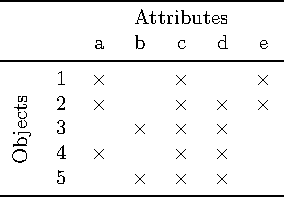
\includegraphics[width=\textwidth,keepaspectratio]{images/background/FCA-conext-ex.pdf}
		\caption{Formal context.}
		\label{fig:example-FC}
	\end{subfigure}
	\hfill
	\begin{subfigure}[b]{0.6\textwidth}
		\centering
		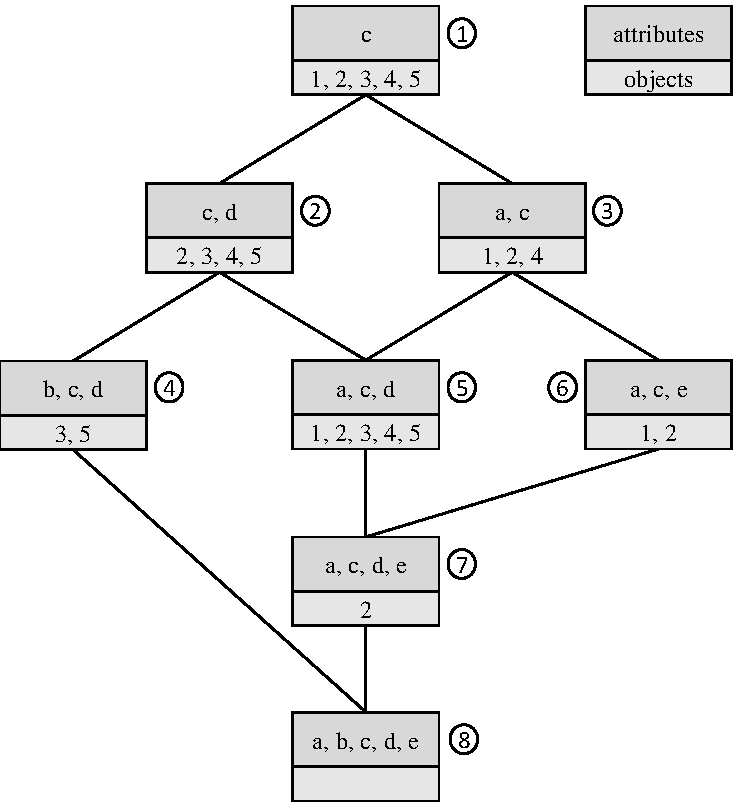
\includegraphics[width=\textwidth,keepaspectratio]{images/background/FCA-lattice-ex.pdf}
		\caption{Concept lattice.}
		\label{fig:example-CL}
	\end{subfigure}
	
	\caption[Example of a formal context in tabular form and corresponding concept lattice]{Example of a formal context in tabular form and corresponding concept lattice. An entry $\times$ in the context table represents that the corresponding object has the corresponding attribute.}
	\label{fig:example-FC-CL}
\end{figure}

%%%%%%%%%%%%%%%%%%%%%%%%%%%%%%%%%%%%%%%%%%%%%%%%%%%%%%%%%%%%%%%%%%%%%%%%
\subsection{Gaussian Mixture Model}\label{sec:GMM}
%%%%%%%%%%%%%%%%%%%%%%%%%%%%%%%%%%%%%%%%%%%%%%%%%%%%%%%%%%%%%%%%%%%%%%%%
A Gaussian mixture model (GMM) is a probability density function represented as the weighted sum of component Gaussian densities  \cite{Reynolds2009}. The mixture represents a normally distributed overall population whereas the components represent subpopulations within the whole population. For one-dimensional data, a GMM with $M$ components can be defined as:
\begin{equation}
	\hat{f}_{GMM}\left(x\right) =  \sum_{m = 1}^{M}\varnothing_{m}\mathcal{N}\left(x\right\vert  \mu_{m},\sigma_{m})
\end{equation}
where, \(\varnothing_{m} \geq 0\) is the mixture weight i.e. the probability of \( m\)-th component \( \kappa_{m}\) satisfying \( \sum_{m = 1}^{M}\varnothing_{m} = 1\)  so that the total probability distribution normalizes to $1$, and \(\mathcal{N}\left(x\right\vert  \mu_{m},\sigma_{m})\) is the distribution of a Gaussian component with mean \( \mu_{m}\) and standard deviation \( \sigma_{m}\) defined as:
\begin{equation}
	\mathcal{N}\left(x\right\vert  \mu_{m},\sigma_{m}) =\frac{1}{\sigma_{m}\sqrt{2\pi }}e^{-\frac{1}{2}\left(\frac{x-\mu_{m}}{\sigma_{m}}\right)^{2}}
\end{equation}

Expectation-Maximization, an iterative unsupervised learning technique can be used to determine the parameters of GMM \cite{Dempster1977}. Steps involved in Expectation-Maximization for \( n\)  data points \( X = \{ x_{t}\vert t = 1,\ldots ,n\}\)  are:
\begin{itemize}
	\item Guess initial values for GMM parameters denoted by \(\hat{\mu }_{m},\hat{\sigma }_{m},\)  and \( \hat{\varnothing }_{m}\)  respectively.
	
	\item  Expectation step: calculate \(\hat{\gamma }_{t,m}\) , the probability of a point \( x_{t}\)  being generated by \( \kappa_{m}\)
	
	\begin{equation}
		\hat{\gamma }_{t,m} = \frac{\hat{\varnothing }_{m}\mathcal{N}\left(x_{t}\right\vert \hat{\mu }_{m},\hat{\sigma }_{m})}{\sum_{r = 1}^{M}\hat{\varnothing }_{r}\mathcal{N}\left(x_{t}\right\vert \hat{\mu }_{r},\hat{\sigma }_{r})}
	\end{equation}
	
	\item Maximization step: Update GMM parameters using the following equations:
	\begin{equation}
		\hat{\mu }_{m} =\frac{\sum_{t = 1}^{n}\hat{\gamma }_{t,m}x_{t}}{\sum_{t = 1}^{n}\hat{\gamma }_{t,m}}
	\end{equation}
	
	\begin{equation}
		\hat{\sigma }_{m} =\sqrt{\frac{\sum_{t = 1}^{n}\hat{\gamma }_{t,m}(x_{t}-\hat{\mu }_{m})^{2}}{\sum_{t = 1}^{n}\hat{\gamma }_{t,m}}}
	\end{equation}
	
	\begin{equation}
		\hat{\varnothing }_{m} = \sum_{t = 1}^{n}\frac{\hat{\gamma }_{t,m}}{n}
	\end{equation}
	
	\item Repeat Expectation and Maximization steps until the total likelihood $L$ converges, where
	\begin{equation}
		L = \prod_{t = 1}^{n}\hat{f}_{GMM}\left(x_{t}\right)
	\end{equation}
\end{itemize}

Information criterion tests like Akaike Information Criteria (AIC) \cite{Akaike1974} and Bayesian Information Criteria (BIC) \cite{Schwarz2007} can be used to select an appropriate GMM by penalizing the number of free parameters to prevent overfitting. AIC and BIC can be defined as:
\begin{equation}
	AIC = 2p+2\ln L
\end{equation}
\begin{equation}
	BIC = p\ln L+2\ln L
\end{equation}
where $p$ is the number of free parameters and $\ln$ is the natural logarithm. The preferred GMM is the one with minimum AIC and BIC values.

%%%%%%%%%%%%%%%%%%%%%%%%%%%%%%%%%%%%%%%%%%%%%%%%%%%%%%%%%%%%%%%%%%%%%%%%
\subsection{Kernel Density Estimation}\label{sec:KDE}
%%%%%%%%%%%%%%%%%%%%%%%%%%%%%%%%%%%%%%%%%%%%%%%%%%%%%%%%%%%%%%%%%%%%%%%%
Kernel density estimation (KDE) is a non-parametric way of estimating the probability density function of an independent and identically distributed random variable \cite{Parzen1962,Rosenblatt1956}. For \( n\)  data points \( X = \{ x_{t}\vert t = 1,\ldots ,n\}\), KDE is calculated as:
\begin{equation}
	\hat{f}_{KDE}\left(x\right) = \frac{1}{nh}\sum_{t = 1}^{n}K\left(\frac{x-x_{t}}{h}\right)
\end{equation}
where \( h\) is the bandwidth and \( K\) is the kernel function. If a Gaussian kernel function is used to estimate the density of univariate data then the bandwidth can be selected using Silverman’s rule of thumb \cite{Silverman2018} as shown in the following equation:
\begin{equation}
	h=0.9 min\left (\hat{\sigma},\frac{IQR}{1.34}\right)n^{\frac{-1}{5}}
\end{equation}
where \( IQR\) is the interquartile range and \(\hat{\sigma }\) is the standard deviation of the samples.


%%%%%%%%%%%%%%%%%%%%%%%%%%%%%%%%%%%%%%%%%%%%%%%%%%%%%%%%%%%%%%%%%%%%%%%%
\subsection{Transfer Learning and Pre-training strategies}\label{sec:TL}
%%%%%%%%%%%%%%%%%%%%%%%%%%%%%%%%%%%%%%%%%%%%%%%%%%%%%%%%%%%%%%%%%%%%%%%%
Transfer learning is a collection of techniques to enhance the performance of a model on a target task using the information that a model acquires during training on a source task, even if the two tasks are dissimilar \cite{5288526}. Transfer learning focuses on knowledge adaptation and it is defined using two concepts: domains and tasks. A domain $\mathcal{D}=\left \{ \mathcal{X},P(X) \right \}$ has two components: A feature space $\mathcal{X}$ and a marginal probability distribution $P(X)$ where $X=\left \{ x_{1},\cdots ,x_{n} \right \} \in \mathcal{X}$. For a domain $\mathcal{D}$ a task $\mathcal{T}=\left \{ \mathcal{Y},f(x) \right \}$ has two parts: A label space $\mathcal{Y}$ and a predictive function $f:\mathcal{X}\rightarrow\mathcal{Y}$, that can be learned from training data of pairs $\left \{ x_{i},y_{i} \right \}$ where $ x_{i} \in X, y_{i} \in \mathcal{Y}$. Pan and Yang \cite{5288526} defined transfer learning as:
\begin{definition}[Transfer Learning]
	\enquote{Given a source domain $\mathcal{D}_S$ and learning task $\mathcal{T}_S$, a target domain $\mathcal{D}_T$ and learning task  $\mathcal{T}_T$, transfer learning aims to help improve the learning of the target predictive function $f_T(\cdot)$ in  $\mathcal{D}_T$ using the knowledge in  $\mathcal{D}_S$ and  $\mathcal{T}_S$, where $\mathcal{D}_S \neq \mathcal{D}_T$, or $\mathcal{T}_S \neq \mathcal{T}_T$} \cite{5288526}.
\end{definition}

\noindent Plested and Gedeon \cite{Plested2022} defined deep transfer learning in the context of image classification as:
\begin{definition}[Deep Transfer Learning]
	\enquote{Given a source domain $\mathcal{D}_S$ and learning task $\mathcal{T}_S$, a target domain $\mathcal{D}_T$ and learning task  $\mathcal{T}_T$, transfer learning aims to help improve the performance of the target model $M$ on the target task $\mathcal{T}_T$ by initializing it with weights $W$ that are trained on source task  $\mathcal{T}_S$ using source dataset $D_{S}$ (pretraining), where $\mathcal{D}_S \neq \mathcal{D}_T$, or $\mathcal{T}_S \neq \mathcal{T}_T$} \cite{Plested2022}.
\end{definition}

Transfer learning can be broadly categorized into three settings based on $\mathcal{T}_S$, $\mathcal{T}_T$ and provided labels as shown in Figure \ref{fig:transfer-learn-taxonomy} \cite{Mao2020, Ruder2019Neural}. If $\mathcal{T}_S = \mathcal{T}_T$ with only source domain labels provided, it is called transductive transfer learning. When  $\mathcal{T}_S \neq \mathcal{T}_T$ with labels available for the target domain, it is called inductive transfer learning. If no labels are provided then it is called unsupervised transfer learning. Inductive transfer learning can be subdivided into multi-task and sequential transfer learning. $\mathcal{T}_S$ and $\mathcal{T}_T$ are simultaneously learned in multi-task learning whereas, in sequential transfer learning  $\mathcal{T}_S$ is first learned (pre-training stage), and then $\mathcal{T}_T$ is learned (fine-tuning stage). In this thesis, we are focusing on sequential transfer learning.
\begin{figure}[htb!]
	\centering
	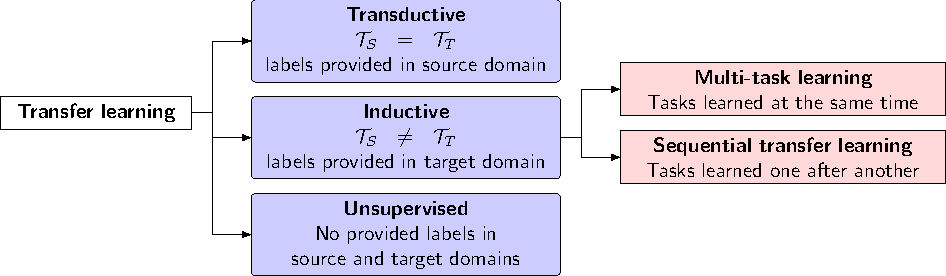
\includegraphics[width=\textwidth,,keepaspectratio]{images/background/transfer-learning-taxonomy.pdf}
	\caption[Transfer learning scenarios]{Transfer learning scenarios \cite{Mao2020, Ruder2019Neural}. $\mathcal{T}_S$ and $\mathcal{T}_T$ represent source and target tasks respectively.}
	\label{fig:transfer-learn-taxonomy}
\end{figure}

Pre-training in the context of transfer learning can be supervised or self-supervised (described in next para) \cite{Mao2020}. Supervised transfer learning uses a pre-trained model that was trained on a sizable dataset for a particular task as a starting point for a new task. A smaller dataset is used to fine-tune the pre-trained model on the new task in order to adapt it to the new task. For instance, a model that has already been trained on a huge image classification dataset like ImageNet \cite{Russakovsky2015} can be fine-tuned for a particular image classification job, like detecting cats vs dogs, on a smaller dataset. This strategy can save resources and shorten the training period and also increase the new model's accuracy.

Self-supervised pre-training uses a model that has already been trained on a related task that does not require labeled data as a starting point for a new task.  In self-supervised pre-training for image classification, the model is first taught to extract important features from images using unsupervised techniques like pretext tasks, generative modeling, or contrastive learning \cite{9462394}. A pretext task can be predicting a specific feature of the data, like predicting an image's rotation or hue. Generative modeling involves training the model to create realistic synthetic data.  Contrastive learning involves training the model to differentiate between negative and positive image pairs. Using this unsupervised pre-training technique the model learns a useful representation of the data which can be refined for a new downstream task on a  labeled dataset. When labeled data is hard to come by or expensive, this strategy can be especially helpful. We can use a source task with a lot of unlabeled examples and transfer the learned knowledge to an interesting target task thanks to the complementing research fields of self-supervised learning and transfer learning \cite{Mao2020}.

%%%%%%%%%%%%%%%%%%%%%%%%%%%%%%%%%%%%%%%%%%%%%%%%%%%%%%%%%%%%%%%%%%%%%%%%
\subsection{Visual Explanation of CNN Model}\label{sec:Grad-CAM}
%%%%%%%%%%%%%%%%%%%%%%%%%%%%%%%%%%%%%%%%%%%%%%%%%%%%%%%%%%%%%%%%%%%%%%%%
Explainability is important for AI tools especially in the case of medical applications \cite{Vellido2020} to understand how a model is taking its decision. Explainability techniques can be model-based (the model itself is explainable i.e. easy to be understood) vs post hoc (explains a trained model), model-specific (limited to particular types of models) vs model-agnostic (independent of the type of the model), and global (provides general relationships learned by the model in a dataset level) vs local (provides explanations for individual input) \cite{VanderVelden2022}. Visual explanation that shows regions of the input image that are significant for predictions from the model is common used for medical image analysis \cite{VanderVelden2022}. Grad-CAM \cite{Selvaraju2020} is a post hoc, model-specific technique for local visual explanation of CNNs. Grad-CAM uses gradient flowing into the ultimate convolution layer for producing heatmaps, and it is a kind of post-hoc attention that can be applied on an already trained model. Grad-CAM provides similar result to occlusion sensitivity map \cite{10.1007/978-3-319-10590-1_53} that works by masking patches of the input image, but Grad-CAM is much faster to calculate compared to image occlusion \cite{Selvaraju2020}.  Grad-CAM has been used for visual explanation in numerous medical image analysis tasks including brain \cite{10.3389/fnins.2020.00630}, breast \cite{ElAdoui2020}, cardiovascular \cite{Candemir2020}, chest \cite{Brunese2020}, dental \cite{8977504}, eye \cite{Martins2020}, female reproductive system \cite{9098587}, gastrointestinal \cite{Itoh2020}, lymph nodes \cite{Ji2019}, musculosketal \cite{VonSchacky2020}, thyroid \cite{Lee2020}, and skin \cite{Zunair2020} images. We utilized Grad-CAM technique for visualizing the regions of the input image that are significant for skin lesion class prediction from the CNN models (as shown in Figure \ref{fig:gradcam-example}) used in our study. 
\begin{figure}[htb!]
	\centering
	\begin{subfigure}[b]{0.4\textwidth}
		\centering
		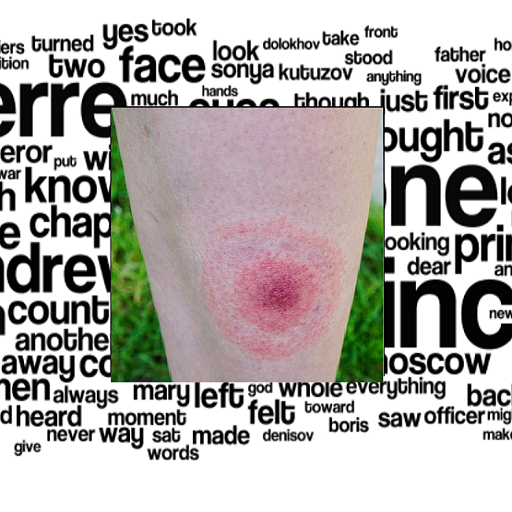
\includegraphics[width=\textwidth,keepaspectratio]{images/pretraining/gradcam/CenteredLyme9.png}
		\caption{Input image.}
		\label{fig:grad-input}
	\end{subfigure}
	\hfill
	\begin{subfigure}[b]{0.4\textwidth}
		\centering
		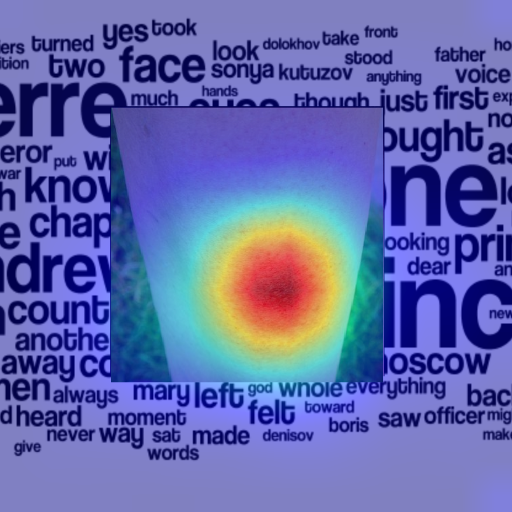
\includegraphics[width=\textwidth,keepaspectratio]{images/pretraining/gradcam/9/EfficientNetB5CombinedGradCam.png}
		\caption{Gard-CAM visualization.}
		\label{fig:grad-result}
	\end{subfigure}
	
	\caption{Gard-CAM visualization example.}
	\label{fig:gradcam-example}
\end{figure}

%%%%%%%%%%%%%%%%%%%%%%%%%%%%%%%%%%%%%%%%%%%%%%%%%%%%%%%%%%%%%%%%%%%%%%%%
\section{Literature Review}\label{sec:litreview}
%%%%%%%%%%%%%%%%%%%%%%%%%%%%%%%%%%%%%%%%%%%%%%%%%%%%%%%%%%%%%%%%%%%%%%%%
The following subsections review the related works on AI for skin lesion diagnosis, a brief overview of Lyme disease with the use of AI for Lyme disease diagnosis, and also the works on the data scarcity problem.
%%%%%%%%%%%%%%%%%%%%%%%%%%%%%%%%%%%%%%%%%%%%%%%%%%%%%%%%%%%%%%%%%%%%%%%%
\subsection{AI for Skin Disorder Diagnosis}
%%%%%%%%%%%%%%%%%%%%%%%%%%%%%%%%%%%%%%%%%%%%%%%%%%%%%%%%%%%%%%%%%%%%%%%%
Many works have been done utilizing deep learning techniques specifically convolutional neural networks (CNNs) for diagnosing cancerous and other common skin lesions from dermoscopic images. Haenssle et al. \cite{Haenssle2018} used transfer learning from ImageNet \cite{Russakovsky2015} pre-trained InceptionV4 CNN architecture for detecting melanoma skin cancer using images from International Skin Imaging Collaboration (ISIC) \cite{Codella2019} dermoscopic image archive and compared the model's performance against 58 dermatologists. CNN outperformed most of the expert dermatologists. Brinker et al. \cite{Brinker2019} also used ImageNet transfer learning with ResNet50 CNN architecture on a dataset of 12,378 dermoscopic images from ISIC archive for the melanoma classification task and compared the CNN's performance against dermatologists. Again deep learning outperformed 136 out of 157 dermatologists. Maron et al. \cite{Maron2019}] also used ResNet50 architecture with ImageNet transfer learning and performed a multiclass cancer classification using 11,444 dermoscopic images from ISIC archive where most of the images were taken from HAM10000 dataset \cite{Tschandl2018}. This study also showed the superiority of deep learning models compared to 112 dermatologists. 

Liu et al. \cite{Liu2020} trained an InceptionV4 based deep learning system using clinical skin lesion images and patient data from 16,114 verified cases for the differential diagnosis of 26 common skin conditions. Esteva et al. \cite{Esteva2017} trained an InceptionV3 CNN architecture on a dataset of 126,076 clinical skin lesion images and 3,374 dermoscopic images using ImageNet transfer learning for skin cancer classification. The deep learning model performed on par compared with 21 board-certified expert dermatologists. Han et al. \cite{Han2018} trained an ensemble model of ResNet152 and VGG19 CNN architectures using a dataset of 49,567 clinical skin lesion images of onychomycosis that outperformed most of the expert dermatologists.

Results from aforementioned studies confirmed that deep learning-based systems compete on par with expert dermatologists for diagnosing diseases from dermoscopic and clinical skin lesion images. Recent studies showed that incorporating data from multiple modalities in the analysis process significantly improves the artificial intelligence based models' performance compared to a single modality based analysis for many medical diagnosis tasks \cite{Senaratne10.1145/3556980, Li10.1145/3344256, Pacheco9364366, Chen2022}. Pacheco et al. \cite{Pacheco9364366} proposed an attention based deep learning approach for combining images and patient data for skin cancer classification that resulted in better performance compared to a single modality based analysis. Chen et al. \cite{Chen2022} showed a 9 percent improvement in model accuracy with a multimodal fusion of skin image and clinical data compared to image only skin cancer classification. 

%%%%%%%%%%%%%%%%%%%%%%%%%%%%%%%%%%%%%%%%%%%%%%%%%%%%%%%%%%%%%%%%%%%%%%%%
\subsection{AI for Lyme Disease Diagnosis}
%%%%%%%%%%%%%%%%%%%%%%%%%%%%%%%%%%%%%%%%%%%%%%%%%%%%%%%%%%%%%%%%%%%%%%%%
Lyme disease is an infectious disease transmitted by ticks and caused by pathogenic bacteria of the \textit{Borrelia burgdorferi} sensu lato group \cite{Shapiro2014}. It is estimated that around 476,000 people in the United States and more than 200,000 people in western Europe are affected by Lyme disease each year \cite{Marques2021}. Most of the time an expanding round or oval red skin lesion known as erythema migrans (EM) becomes visible in the victim’s body which is the most common early symptom of Lyme disease \cite{Shapiro2014, Burlina2018}. EM usually appears at the site of a tick bite after one to two weeks (range, 3 to 30 days) as a small redness and expands almost a centimeter per day, creating the characteristic bull’s-eye pattern as shown in Figure \ref{fig:EM-bullseye} \cite{Shapiro2014, Burlina2018, Strle2009, Berglund1995}. EM generally vanishes within a few weeks or months but the Lyme disease infection advances to affect the nervous system, skin, joints, eyes, and heart \cite{Shapiro2014, Strle2009}. Antibiotics can be used as a medium of effective treatment in the early stage of Lyme disease. So, early recognition of EM is extremely important to avoid long-term complications of Lyme disease. 

Most European and North American guidelines recommend a two-tier serology test to detect antibodies against \textit{Borrelia burgdorferi} sensu lato for diagnosing Lyme disease \cite{Eldin2019, Trevisan2020}. However, a serology test is only recommended in the absence of EM because early serology has low sensitivity (40\% to 60\%) and may result in false negatives \cite{Eldin2019}. Alternatively, direct detection of Borrelia burgdorferi sensu lato can be done using culture, microscopy, or PCR \cite{Trevisan2020}. The gold standard of microbiological diagnosis - the culture of bacteria requires laboratory expertise and special media for \textit{Borrelia burgdorferi} sensu lato \cite{Eldin2019}. Light microscopy-based detection is not feasible in clinical practice \cite{Trevisan2020}. PCR based diagnosis is also very difficult and shows highly variable sensitivity \cite{Trevisan2020}. Direct detection methods are not always feasible for clinicians because of extended processing time and required expertise \cite{Burlina2020}. The diagnosis of EM is a challenging task because EM can create different patterns instead of the trademark bull’s-eye pattern as shown in Figure \ref{fig:EM-atypical}.

Despite the vast application of AI in the field of skin lesion diagnosis, there are only a few works related to Lyme disease detection from EM skin lesion images. The unavailability of reliable public EM datasets as a result of privacy concerns of medical data may be the reason for the lack of extensive studies in this field. The only publicly available dataset of EM is a small collection of web-scraped unverified images hosted in a kaggle repository \cite{LymeDatasetKaggle}. Čuk et al. \cite{Cuk2014} proposed a visual system for EM recognition on a private EM dataset using classical machine learning techniques including naïve Bayes, SVM, boosting, and neural nets (not deep learning). They considered ellipse, the common shape of EM, and used eccentricity, small and large axis ratio, ellipse angular, and ellipse focus attributes for classification. Deep learning techniques learn image features from training images via an optimization process and recent studies show that image features extracted by deep learning techniques outperform human-engineered image features for medical image classification tasks \cite{Burlina2020}. Burlina et al. \cite{Burlina2018} created a dataset of EM by collecting images from the internet and trained a CNN architecture ResNet50 as a binary classifier to distinguish between EM and other skin conditions. Although their dataset is not public, the trained model is publicly available. Burlina et al. \cite{Burlina2020} further enriched the dataset with more images from the East Coast and Upper Midwest of the United States and trained six CNNs namely ResNet50, InceptionV3, MobileNetV2, DenseNet121, InceptionResNetV2, and ResNet152 for EM classification. They did not make the dataset or the trained models public for the extended study. Burlina et al. \cite{Burlina2018} and Burlina et al. \cite{Burlina2020} used transfer learning from ImageNet pre-trained models and studied the CNNs in terms of predictive performance. Koduru et al. \cite{Koduru2021} deployed a trained ResNet50 CNN model utilizing a private dataset  for a prototype application to identify EM. Jacob et al. \cite{Jacob2022} used the kaggle Lyme dataset \cite{LymeDatasetKaggle} to test state-of-the-art self-supervised learning techniques against supervised transfer learning for different CNN architectures and comparatively self-supervised learning underperformed. Oholtsov et al. \cite{Oholtsov2023} suggested using both clean and dirty images for training EM classifier based on experimentation using an unverified dataset of only 106 EM images.

\begin{figure}[htb!]
	\centering
	\begin{subfigure}[b]{0.4\textwidth}
		\centering
		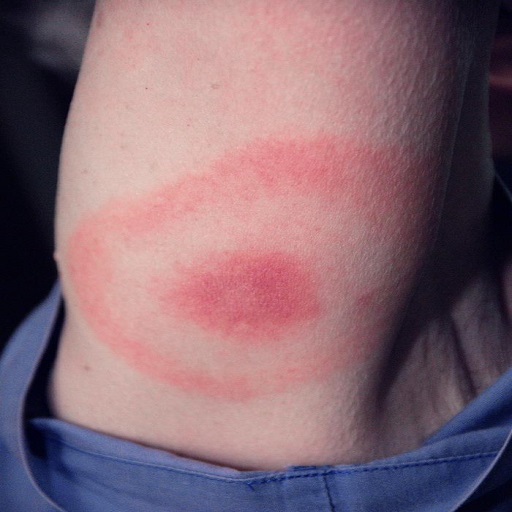
\includegraphics[width=\textwidth,keepaspectratio]{images/background/EM_bullseye.jpg}
		\caption{Bull’s-eye pattern.}
		\label{fig:EM-bullseye}
	\end{subfigure}
	\hfill
	\begin{subfigure}[b]{0.4\textwidth}
		\centering
		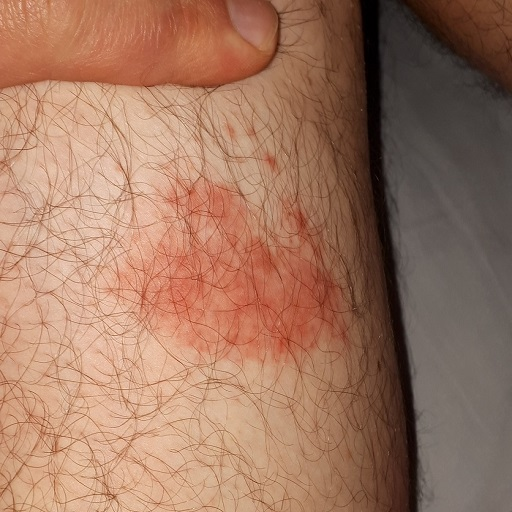
\includegraphics[width=\textwidth,keepaspectratio]{images/background/EM_atypical.jpg}
		\caption{Atypical pattern.}
		\label{fig:EM-atypical}
	\end{subfigure}
	
	\caption[Patterns of erythema migrans]{Patterns of erythema migrans (EM) \cite{EMPatterns}.}
	\label{fig:EM-patterns}
\end{figure}

%%%%%%%%%%%%%%%%%%%%%%%%%%%%%%%%%%%%%%%%%%%%%%%%%%%%%%%%%%%%%%%%%%%%%%%%
\subsection{Related Works on Data Scarcity}\label{RelWorkDataScarcity}
%%%%%%%%%%%%%%%%%%%%%%%%%%%%%%%%%%%%%%%%%%%%%%%%%%%%%%%%%%%%%%%%%%%%%%%%
Transfer learning and expanding data by transforming images with augmentation techniques are frequently used by researchers to improve deep learning model's performance on limited image datasets. Perez et al \cite{Perez2018} showed that using data augmentation significantly improves model's performance using InceptionV4, ResNet, and DenseNet architectures for melanoma classification with dermoscopic images from ISIC archive. P{\'{e}}rez et al. \cite{Perez2021} showed that combining transfer learning and data augmentation significantly improves model's performance for melanoma diagnosis from images using an extensive experimental study on 11 datasets and 12 CNN architectures. 

Transfer learning with supervised ImageNet\cite{Russakovsky2015} pre-training is frequently used in medical image analysis tasks \cite{10.1117/12.2531198, 7950523, McKinney2020, Liu2020, Graziani2019VisualizingAI, Heker2020}. Transfer learning from natural images of ImageNet provides performance improvement according to multiple empirical studies \cite{app10134523, Graziani2019VisualizingAI, Heker2020}. Even if this strategy does not guarantee an improvement in performance Raghu et al. \cite{Raghu2019} showed using a detailed study that it speeds up convergence and is especially helpful for training with limited data. Gu et al. \cite{GuRef} showed that progressive transfer learning starting from an ImageNet pre-trained model end-to-end fine-tuned on a dataset of similar skin lesions with a slight domain shift increases the classification performance of skin cancer classification task for a smaller dataset. Recently, self-supervised pre-training using unlabeled domain-specific data is gaining popularity in medical image analysis \cite{9710396, He2020.04.13.20063941, 9010639, 10.1007/978-3-030-59710-8_39, https://doi.org/10.48550/arxiv.2211.08559, https://doi.org/10.48550/arxiv.2010.05352}. Azizi et al. \cite{9710396} showed that training a model on ImageNet in self-supervised fashion followed by self-supervised learning on unlabeled in-domain medical images, and fine-tuning end-to-end for downstream supervised tasks significantly improves model accuracy. They used ResNet architectures on X-ray and dermatology classification tasks for experimentation. Dadsetan et al. \cite{https://doi.org/10.48550/arxiv.2211.08559} also showed that combining ImageNet and domain-specific self-supervised pre-training gives better performance for Alzheimer's disease propagation from brain magnetic resonance imaging.

For multimodal training i.e. training utilizing all the available modalities (for example, image modality and patient data modality), the general assumption is that both the training and test data will have full and paired modalities \cite{ngiam2011multimodal,Zadeh2017}. However, missing data is common for real-world clinical scenarios \cite{Huang2020}. Existing works in the literature generally drop the incomplete samples or impute missing values \cite{ma2021smil, 10.1145/3534678.3539388}. Some studies report improvements by dropping incomplete samples \cite{10.1145/3308558.3313643, wang2020multimodal}. Generative models are used in many studies for imputing missing modalities \cite{LI2020105592, 10.1145/3219819.3219963, pan2021disease}. Ma et al. \cite{ma2021smil} approximated missing modality using modality priors learned from dataset. Chen et al. \cite{10.1145/3394486.3403182} fused multimodal incomplete data using a heterogeneous graph structure. Zhang et al. \cite{10.1145/3534678.3539388} considered auxiliary data from similar neighbors of a patient to deal with missing modalities. If paired data is missing for the modalities but training data for individual modalities are available then individual classifiers can be trained for each modality and the results can be fused using a weighing scheme \cite{rahate2022multimodal}.

%%%%%%%%%%%%%%%%%%%%%%%%%%%%%%%%%%%%%%%%%%%%%%%%%%%%%%%%%%%%%%%%%%%%%%%%


\section{Research Questions and Challenges}\label{sec:research-questions}
%%%%%%%%%%%%%%%%%%%%%%%%%%%%%%%%%%%%%%%%%%%%%%%%%%%%%%%%%%%%%%%%%%%%%%%%
Pre-training with in-domain images is effective for increasing the performance of deep CNN based image classifiers however it is difficult to collect a large number of in-domain images for many skin conditions like EM. The dataset created as part of our study for EM analysis consists of clinical skin lesion images. First, we thought of pre-training a CNN for EM classification using clinical skin lesion images of other skin lesions as we could not collect a large number of in-domain unlabeled samples related to EM. Most of the accessible datasets are concerned with skin cancers. Wen et al. \cite{WEN2022e64} systematically reviewed the available datasets for skin cancers. Out of the open access clinical skin lesion image datasets, SD-198 \cite{sun2016benchmark} containing 6,584 clinical skin lesion images and its extended version SD-260 \cite{8736039} containing 20,600 clinical skin lesion images of skin cancer images seemed promising but these datasets are not easily accessible \footnote{ The download link mentioned in the paper did not work and we did not get any response from the authors after asking for access.}. On the contrary, dermoscopic image datasets like HAM10000 dataset \cite{Tschandl2018} are easily accessible. The image modality of clinical EM dataset is quite different from dermoscopic images of HAM10000 dataset as shown in Figure \ref{fig:EM-bullseye2} and \ref{fig:dermo-sample}. Our first research question is:
%\begin{tcolorbox}[width=\textwidth]   
\begin{researchquestion}\label{question1}
	Can we improve the performance of ImageNet pretrained clinical skin lesion image classifier's performance with additional pre-training using dermoscopic images?
\end{researchquestion}
%\end{tcolorbox} 

\begin{figure}[htb!]
	\centering
	\begin{subfigure}[b]{0.3\textwidth}
		\centering
		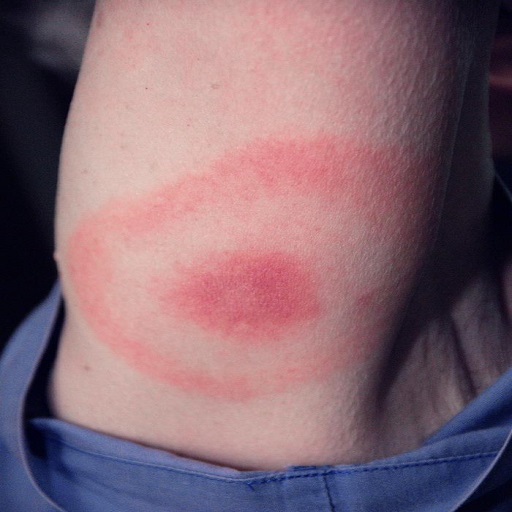
\includegraphics[width=\textwidth,keepaspectratio]{images/background/EM_bullseye.jpg}
		\caption{Clinical image.}
		\label{fig:EM-bullseye2}
	\end{subfigure}
	\hfill
	\begin{subfigure}[b]{0.3\textwidth}
		\centering
		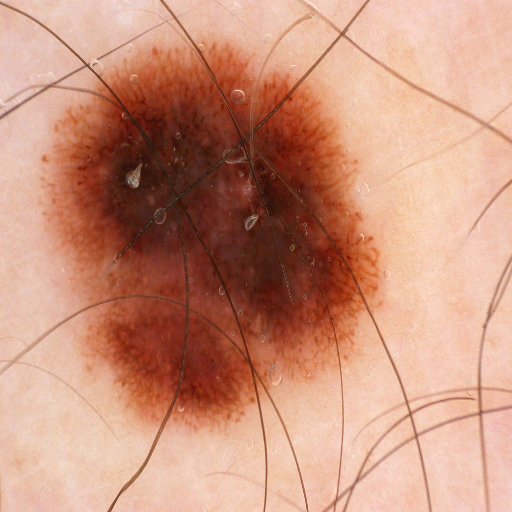
\includegraphics[width=\textwidth,keepaspectratio]{images/background/dermoscopic_sample.png}
		\caption{Dermoscopic image.}
		\label{fig:dermo-sample}
	\end{subfigure}
	\hfill
	\begin{subfigure}[b]{0.3\textwidth}
		\centering
		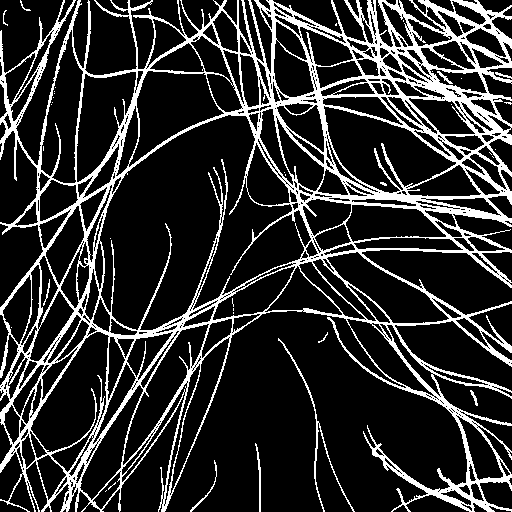
\includegraphics[width=\textwidth,keepaspectratio]{images/background/hair_mask_sample.png}
		\caption{Skin lesion hair mask.}
		\label{fig:hair-mask-sample}
	\end{subfigure}
	
	\caption[Clinical image vs dermoscopic image and a sample of skin lesion hair mask.]{Clinical image of erythema migrans \cite{EMPatterns} vs demoscopic image of skin cancer \cite{Tschandl2018} and a sample of skin lesion hair mask.}
	\label{fig:clinical-vs-dermo}
\end{figure}


Incorporating data from multiple modalities in the analysis process significantly improves the models' performance for skin lesion analysis tasks. For some diseases like Lyme disease, a proper diagnosis based on skin lesions is not effective without considering additional context from patient data. Existing works on early Lyme disease prediction using artificial intelligence techniques only utilize images of EM skin lesions whereas doctors believe corresponding patient data should also be considered to strengthen the predictive performance \cite{Burlina2020,Hossain2022}. Training a multimodal deep learning model utilizing both images and patient data requires a dataset of lesion images with associated patient data. Even though EM image datasets are available, creating a dataset with patient data linked with each lesion image would take much time. Moreover, patient data-only datasets that can be used for creating individual classifiers for Lyme disease are not readily available. So, our second research question is:
%\begin{tcolorbox}[width=\textwidth]    
\begin{researchquestion}\label{question2}
	How to assist deep learning based skin lesion image classifier with patient data in the absence of training data?
\end{researchquestion}
%\end{tcolorbox} 

Occlusion of skin lesions in dermoscopic images due to hair artifacts (as shown in Figure \ref{fig:dermo-sample}) affects the performance of computer-assisted lesion analysis algorithms. To tackle this issue, researchers are working on digital hair segmentation, removal, and augmentation techniques \cite{Attia2020,Li2021}. Standard image processing based hair removal is not beneficial for real-time application and removing hair does not give new features to the network. Augmenting images with skin hair can be of interest. Skin hair augmentation techniques require a hair mask to generate hair in given locations as shown in Figure \ref{fig:hair-mask-sample} \cite{Attia2020}. These masks are created either manually, with random curves or lines and segmentation \cite{Attia2020}. Generative models can be utilized to automate the creation of hair masks. So, our third research question is:
%\begin{tcolorbox}[width=\textwidth]  
\begin{researchquestion}\label{question3}
	How to efficiently deal with skin lesion hair artifacts for AI-assisted analysis of dermoscopic skin lesion images?
\end{researchquestion}
%\end{tcolorbox} 

\section{Conclusion}
%%%%%%%%%%%%%%%%%%%%%%%%%%%%%%%%%%%%%%%%%%%%%%%%%%%%%%%%%%%%%%%%%%%%%%%%
In this chapter, we have provided all the theoretical backgrounds needed to understand the rest of the thesis. In addition, we presented a detailed review of existing works in the literature and framed our research questions in the context of existing works. The following chapters describe our contributions by addressing the research questions presented in this chapter. 
\begin{tcolorbox}[enhanced,attach boxed title to top center={yshift=-3mm,yshifttext=-1mm},
	coltitle=black, colback=blue!5!white,colframe=blue!75!black,colbacktitle=violet!50!white,
	title=Key Points (Chapter \ref{chap:background}),fonttitle=\bfseries,
	boxed title style={colframe=black} ]
	In this thesis, we are addressing three research questions:
	\begin{itemize}
		\item Can we improve the performance of ImageNet pretrained clinical skin lesion image classifier's performance with additional pre-training using dermoscopic images?
		\item How to assist deep learning based skin lesion image classifier with patient data in the absence of training data?
		\item How to efficiently deal with skin lesion hair artifacts for AI-assisted analysis of dermoscopic skin lesion images?
	\end{itemize}
\end{tcolorbox}
